The space of possible kernel composition is infinite. Combining inference over this space with the problem of finding a good parameterization that could potentially explain the observed data best poses a hard problem. The natural language interpretation of the meaning of a kernel and its composition renders this a problem of symbolic computation. Duvenaud and colleagues note that a sum of kernels can be interpreted as logical OR operations and kernel multiplication as logical AND~\citeyearpar{duvenaud2013structure}. This is due to the kernel rendering two points similar if $k_1$ OR $k_2$ outputs a high value in the case of a sum. Respectively, multiplication of two kernels results in high values only if $k_1$ AND $k_2$ have high values (see Fig. \ref{fig:composite} examplifies how to interpret global vs. local aspects and its symbolic analog respectively). 
In the following, we will refer to covariance functions that are not composite as base covariance functions.

\begin{figure}
\centering

\usetikzlibrary{arrows}


\begin{tikzpicture}[->,>=stealth',level/.style={sibling distance = 5cm/#1,
  level distance = 4.5cm}] 
\node [   align=left] {
                   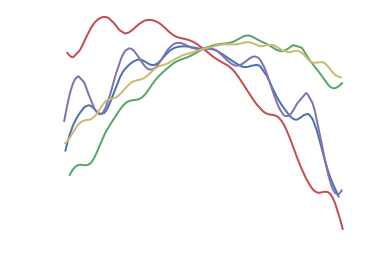
\includegraphics[width=.33\textwidth]{figs/gpSamples/main.png}
\\
SE $\times$ LIN $+$ PER $\times$ LIN $+$  RQ $\times$ LIN}
      child{ node [  align=center]{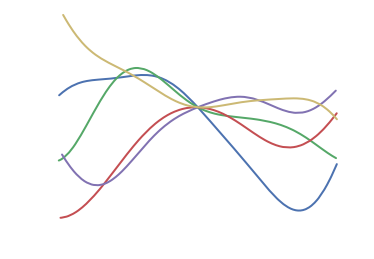
\includegraphics[width=.33\textwidth]{figs/gpSamples/selin.png}\\ SE $\times$ LIN} 
	      child{ node [   align=center] {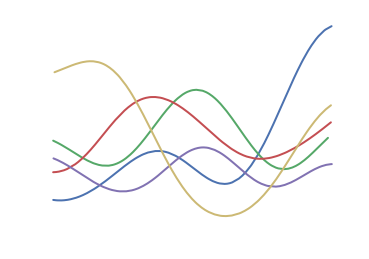
\includegraphics[width=.2\textwidth]{figs/gpSamples/se.png}\\ SE}}
	      child{ node [   align=center] {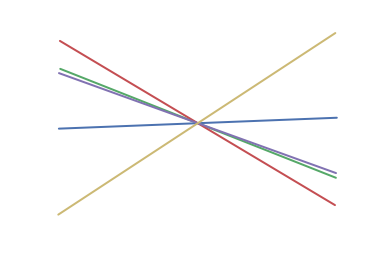
\includegraphics[width=.2\textwidth]{figs/gpSamples/lin.png}\\ LIN }}                            
      }
        child{ node [  align=center]{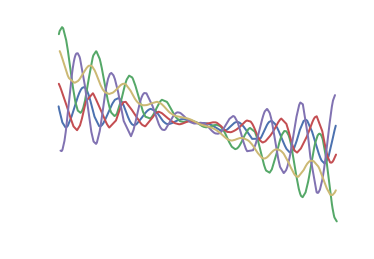
\includegraphics[width=.33\textwidth]{figs/gpSamples/perlin.png}\\ PER $\times$ LIN} 
            child{ node [   align=center] {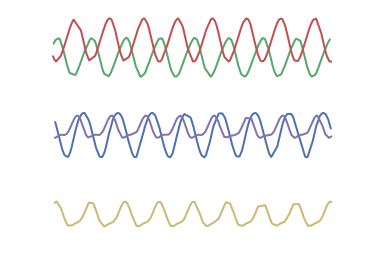
\includegraphics[width=.2\textwidth]{figs/gpSamples/per.png}\\ PER}} 
            child{ node [   align=center] {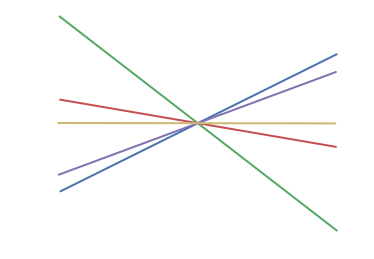
\includegraphics[width=.2\textwidth]{figs/gpSamples/lin2.png}\\ LIN}}
		}
      child{ node [  align=center]{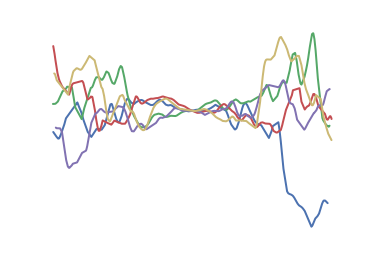
\includegraphics[width=.33\textwidth]{figs/gpSamples/rqlin.png}\\ RQ $\times$ LIN} 
            child{ node [   align=center] {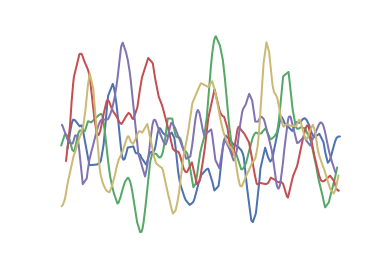
\includegraphics[width=.2\textwidth]{figs/gpSamples/rq.png}\\ RQ}}
            child{ node [   align=center] {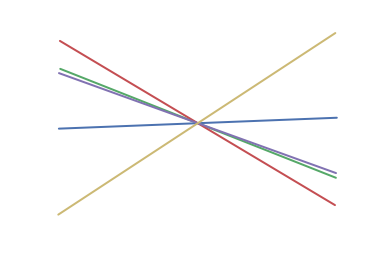
\includegraphics[width=.2\textwidth]{figs/gpSamples/lin.png}\\ LIN}}
		}
; 
\end{tikzpicture}

\caption{Composition of covariance function parsed using the example SE $\times$ LIN $+$ PER $\times$ LIN $+$  RQ $\times$ LIN}\label{fig:composite}
\end{figure}


Knowledge about the composite nature of covariance functions is not new, however, until recently, the choice and the composition of covariance functions were done ad-hoc. The Automated Statistician Project came up with an approximate search over the possible space of kernel structures~\citep{duvenaud2013structure,lloyd2014automatic}. However, a fully Bayesian treatment of this was not done before.
The case where the covariance structure is not given is even more interesting. Our probabilistic programming based MCMC framework approximates the following intractable integrals of the expectation for the prediction:
\begin{equation}
\mathbb{E}[y^* \mid x^*,\mathbf{D},\mathbf{K}] =\iint f(x^*,\bm{\theta},\mathbf{K})\,P(\bm{\theta} \mid \mathbf{D,\mathbf{K}})\,P(\mathbf{K}|\bm{\Omega},s,n) \; \mathbf{d} \bm{\theta} \mathbf{d} \mathbf{K}.  
\end{equation}
This is done by sampling from the posterior probability distribution of the hyper-parameters and the possible kernel:
\begin{equation}
y^* \approx \frac{1}{T} \sum^T_{t=1} f(x^* | \bm{\theta}^{(t)},\mathbf{K}^{(t)}). 
\end{equation}


In order to provide the sampling of the kernel, we introduce a stochastic process to the SP that simulates the grammar for algebraic expressions of covariance function algebra:
\begin{equation}
\mathbf{K}^{(t)} \sim  P(\mathbf{K} \mid \bm{\Omega},s,n)
\end{equation}
Here, we start with a set of possible kernels and draw a random subset. For this subset of size $n$, we sample a set of possible operators that operate on the base kernels. 

The marginal probability of a kernel structure which allows us to sample  is characterized by the probability of a uniformly chosen subset of the set of $n$ possible covariance functions times the probability of sampling a global or a local structure which is given by a binomial distribution: 

\begin{equation}
P(\mathbf{K} \mid \bm{\Omega},s,n) = P(\bm{\Omega} \mid s,n)\times P(s \mid n) \times P(n),
\end{equation}
with
\begin{equation}
P(\bm{\Omega} \mid s,n)= {n \choose r}  p_{+\times}^k (1 - p_{+\times})^{n-k}
\end{equation}
and
\begin{equation}
\label{eq:subsets}
P(s \mid n) = \frac{n!}{ \mid s \mid !}
\end{equation}
where $P(n)$ is a prior on the number of base kernels used which can sample from a discrete uniform distribution. This will strongly prefer simple covariance structures with few base kernels since individual base kernels are more likely to be sampled in this case due to (\ref{eq:subsets}). Alternatively, we can approximate a uniform prior over structures by weighting $P(n)$ towards higher numbers. It is possible to also assign a prior for the probability to sample global or local structures, however, we have assigned complete uncertainty to this with the probability of a flip $p = 0.5$.



Many equivalent covariance structures can be sampled due to covariance function algebra and equivalent representations with different parameterization~\citep{lloyd2014automatic}. Certain covariance functions can differ in terms of the hyper-parameterization but can be absorbed into a single covariance function with a different parameterization. To inspect the posterior of these equivalent structures we convert each kernel expression into a sum of products and subsequently simplify. Rules for this simplification can be found in appendix B.


For reproducing results from the Automated Statistician Project in a Bayesian fashion we first define a prior on the hypothesis space. Note that, as in the implementation of the Automated Statistician, we upper-bound the complexity of the space of covariance functions we want to explore. We also put vague priors on hyper-parameters.

\begin{minipage}{\linewidth}
\small
\belowcaptionskip=-10pt
\begin{lstlisting}[frame=single,mathescape,label=alg:structureVent,basicstyle=\selectfont\ttfamily,numbers=none]
// GRAMMAR FOR KERNEL STRUCTURE
assume base_kernels = list(se, wn, lin, per, rq) // defined as above

// prior on the number of kernels
assume p_number_k = tag(quote(number_kernels), 0, uniform_structure(n))
assume s = tag(quote(choice_subset), 0, subset(base_kernels, p_number_k))

assume cov_compo = proc(l) {
  // kernel composition
  if (size(l) <= 1)
  then { first(l) }
  else { if (flip()) then { add_funcs(first(l), cov_compo(rest(l))) }
                     else { mult_funcs(first(l), cov_compo(rest(l))) }
       }
  }
                          
assume K = tag(quote(composit), 0, cov_compo(s))

assume (f_compute f_emu) = gpmem(f_restr, K)
predict mapv(f_compute(get_data_xs)) // probe all data points

// PERFORMING INFERENCE  
infer  repeat(2000, do(
                        mh(quote(number_kernel), one, 1),
                        mh(quote(choice_subset), one, 1),
                        mh(quote(composit), one, 1),
                        mh(quote(hyper), one, 10)))
\end{lstlisting}

\end{minipage}




We defined the space of covariance structures in a way allowing us to reproduce results for covariance function structure learning as in the Automated Statistician. This lead to coherent results, for example for the airline data set describing monthly totals of international airline passengers (\citealp{box2011time}, according to \citealp{duvenaud2013structure}. The sample is identical with the highest scoring result reported in previous work using a search-and-score method~\citep{duvenaud2013structure} for the CO$_2$ data set (see \citealp{rasmussen2006gaussian} for a description) and the predictive capability is comparable. However, the components factor in a different way due to different parameterization of the individual base kernels. We see that that the most probable alternatives for a structural description both recover the data dynamics (Fig. \ref{fig:posterior_twosamples} for the airline data set).

\begin{comment}
\begin{figure}
        \centering
        \begin{subfigure}[b]{\textwidth} \centering
                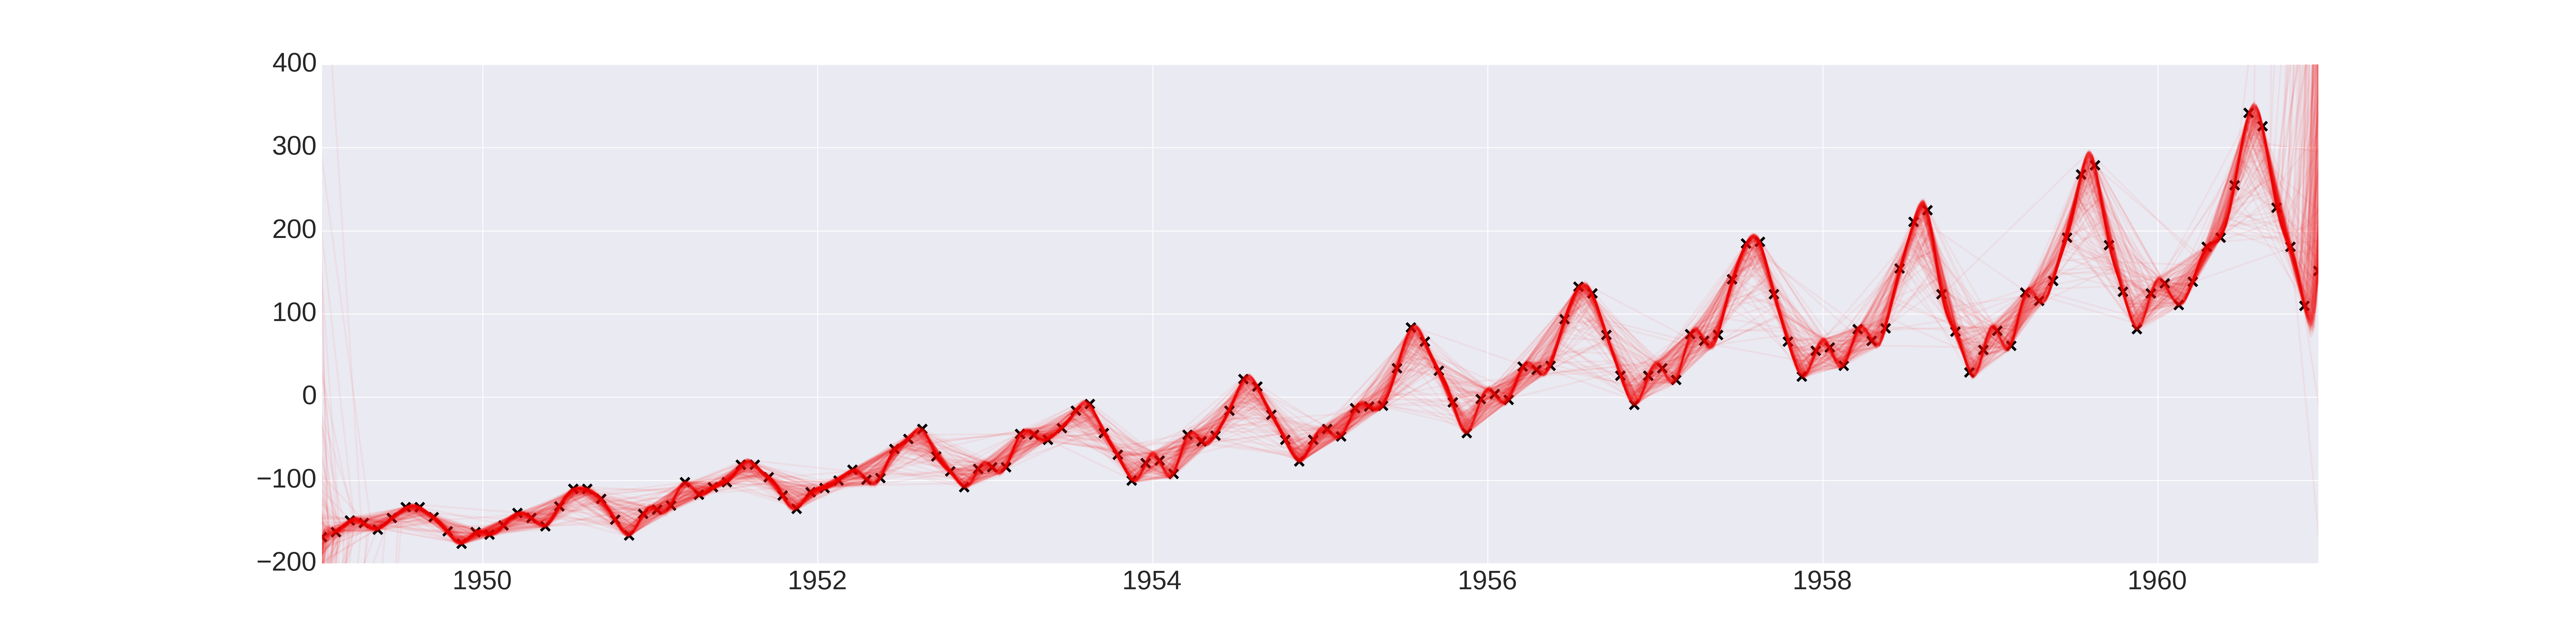
\includegraphics[height=3cm]{figs/airline_tree_3x.png}
                \caption{The predictive posterior using the full grammar structure.}
                \label{fig:airlineBO}
        \end{subfigure}%
        ~ %add desired spacing between images, e. g. ~, \quad, \qquad, \hfill etc.
          %(or a blank line to force the subfigure onto a new line)
          
        \begin{subfigure}[b]{\textwidth} \centering
                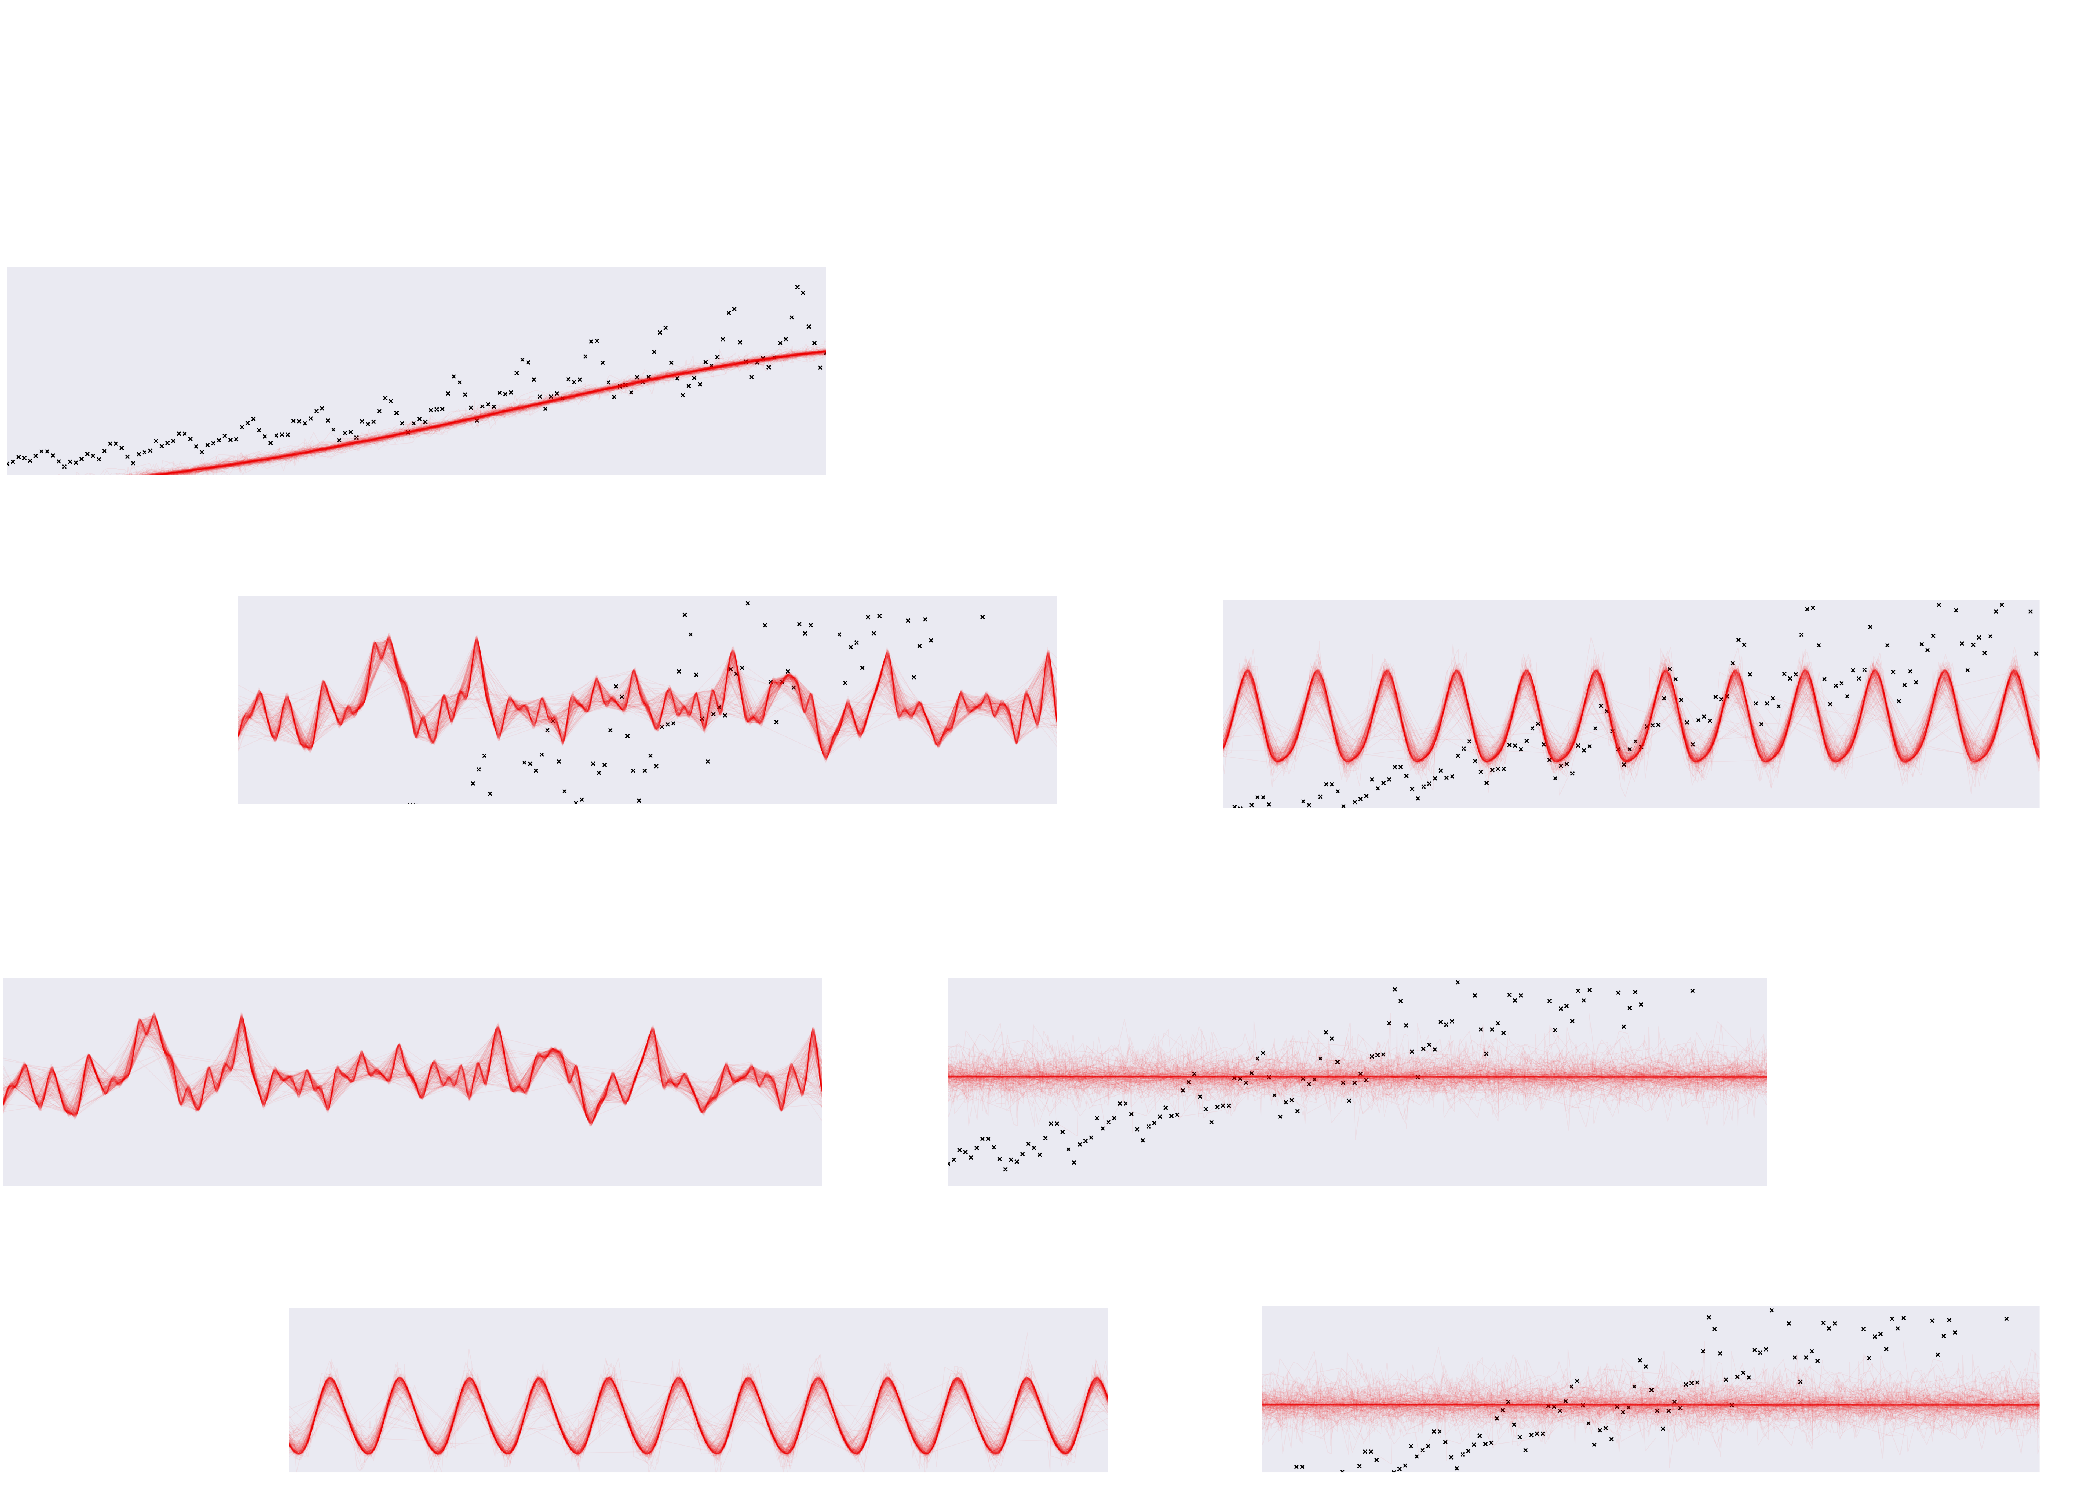
\includegraphics[width=\textwidth]{figs/grammar_tutorial2.png}
                \caption{Compositional Structure}
                \label{fig:AirlineA))}
        \end{subfigure}
        \put(-270,280){SE $\times$ LIN + SE $\times$ LIN (RQ + PER ) $\;\;\; = $} 
        \put(-271,269){\rotatebox{90}{\Large $\Bigg\{$}} 
        \put(-250,267){\vector(-3,-1){30}}
        \put(-220,230){{\Large $+\;\;\;\;\;\;$}SE $\times$ (LIN $\times$ RQ + LIN $\times$ PER) $\;\;\; = $} 
        \put(-395,165){SE {\Large $\times$ \bigg(}} 
        \put(-5,165){\Large \bigg)} 
        \put(-185,165){\Large $+$} 
        \put(-230,146){\vector(0,-1){10}}
        \put(-20,146){\line(0,-1){78}}
        \put(-20,68){\vector(-1,0){150}}
        \put(-251,130){\rotatebox{270}{\Large $\Bigg\{$}} 
        \put(-235,95){\Large $\times$} 
        \put(-191,67){\rotatebox{270}{\Large $\Bigg\{$}} 
        \put(-175,33){\Large $\times$} 
        \caption{a) We see the predictive posterior as a result 1000 nested MH steps on the airline data set. b) depicts a decomposition of this posterior for the structures sampled by Venture. RQ is the rational quadratic covariance function. The first line shows the global trend and denotes the rest of the structure that is shown above. In the second line, the see the periodic component on the right hand side. The left hand side denotes short term deviations both multiplied by a smoothing kernel. The third and fourth lines denote how we reach the second line: both periodic and rational quadratic covariance functions are multiplied by a linear covariance function with slope zero.}\label{fig:tutorial}
\end{figure}
\end{comment}

\begin{figure}
        \centering
        \begin{subfigure}[b]{\textwidth} \centering
                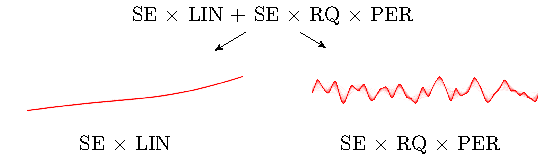
\includegraphics[width=0.65\textwidth]{figs/airline_struct_1.pdf}\caption{}
        \end{subfigure}\\
        
        \vspace*{0.75cm}
	\begin{subfigure}[b]{\textwidth} \centering
                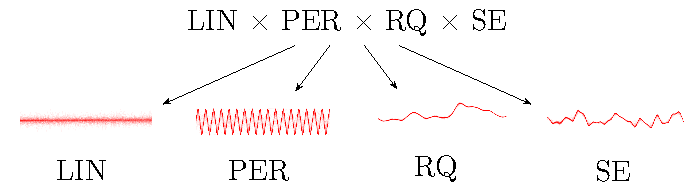
\includegraphics[width=0.6\textwidth]{figs/airline_struct_2.pdf}\caption{}
        \end{subfigure}%
        \caption{(a) most frequent sample drawn from the posterior on structure. We have found two global components. First, A smooth trend (LINxSE) with a non-linear increasing slope. Second, a periodic component with increasing variation and noise. (b) second most frequent sample drawn from the posterior on structure. We found one global component. It is comprised of local changes that are periodic and with changing variation.}\label{fig:posterior_twosamples}
\end{figure}
We further investigated the quality of our stochastic processes by running a leave one out cross-validation computing residuals to gain confidence on the posterior.

\begin{comment}
\begin{figure}
\centering
    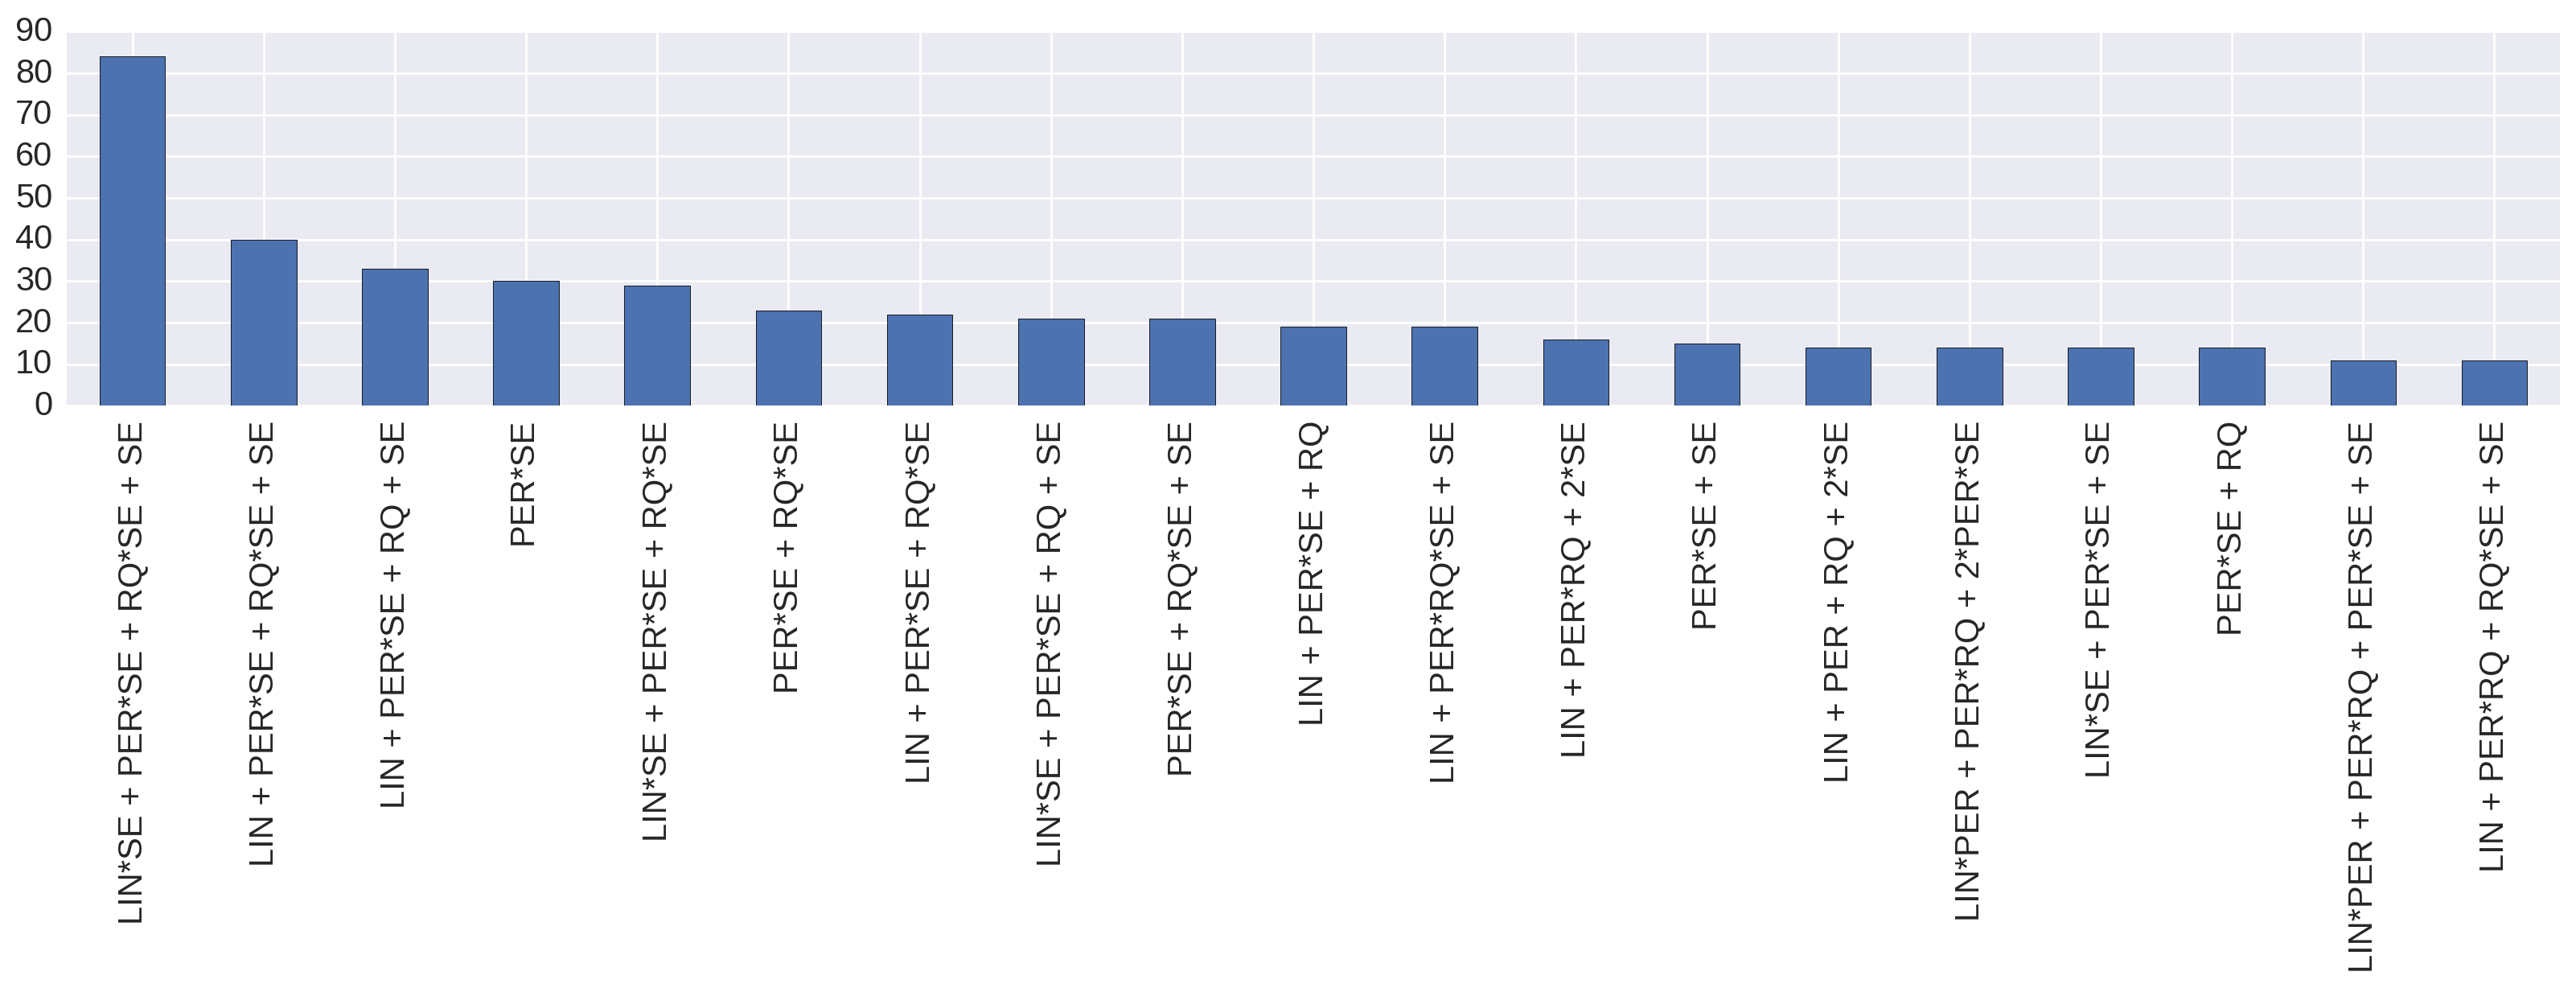
\includegraphics[width=\textwidth]{figs/structureCo2b.png}
    \caption{Posterior on structure of the CO2 data. We have cut the tail of the distribution for space reasons since the number of possible structures is large. We see the final sample of the each of the 545 chains with 2000 nested steps each. Note that \citet{duvenaud2013structure} report LIN $\times$ SE $+$ PER $\times$ SE $+$ RQ $\times$ SE.}\label{fig:structureCo2}
\end{figure}

\begin{figure}
\centering
    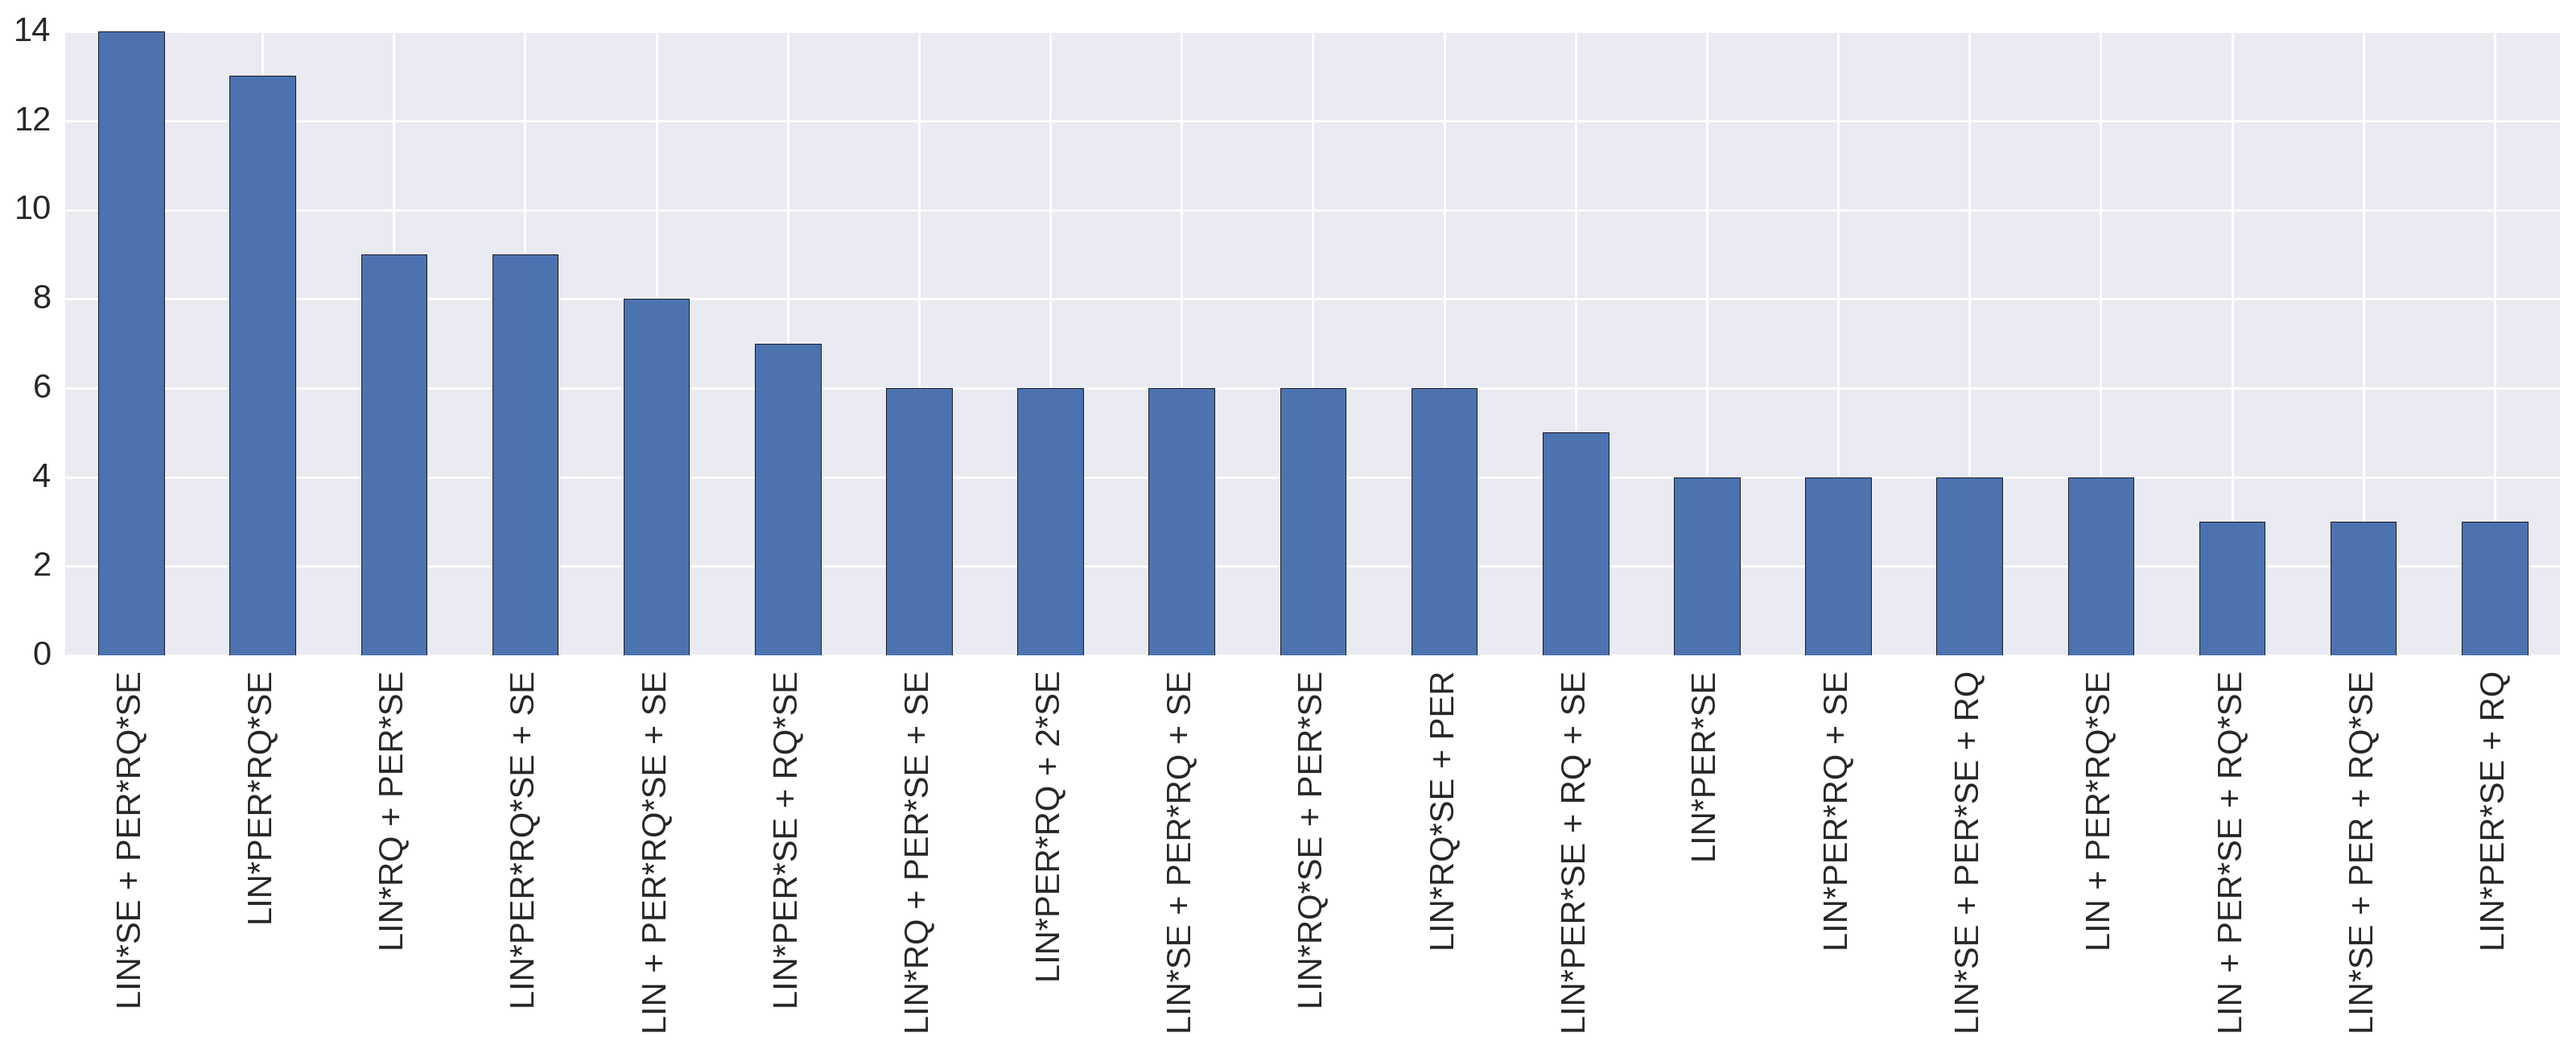
\includegraphics[width=\textwidth]{figs/structureAirlinec.png}
    \caption{Posterior on structure of airline data set. We have cut the tail of the distribution for space reasons since the number of possible structures is large. We see the final sample of the each of the 144 chains with 2000 nested steps each. Note that \citet{duvenaud2013structure} report LIN $\times$ SE $+$ (PER  + RQ) $\times$ SE $\times$ LIN}\label{fig:structureAir}
\end{figure}


\begin{figure}
        \centering
        \begin{subfigure}[b]{0.5\textwidth} \centering
                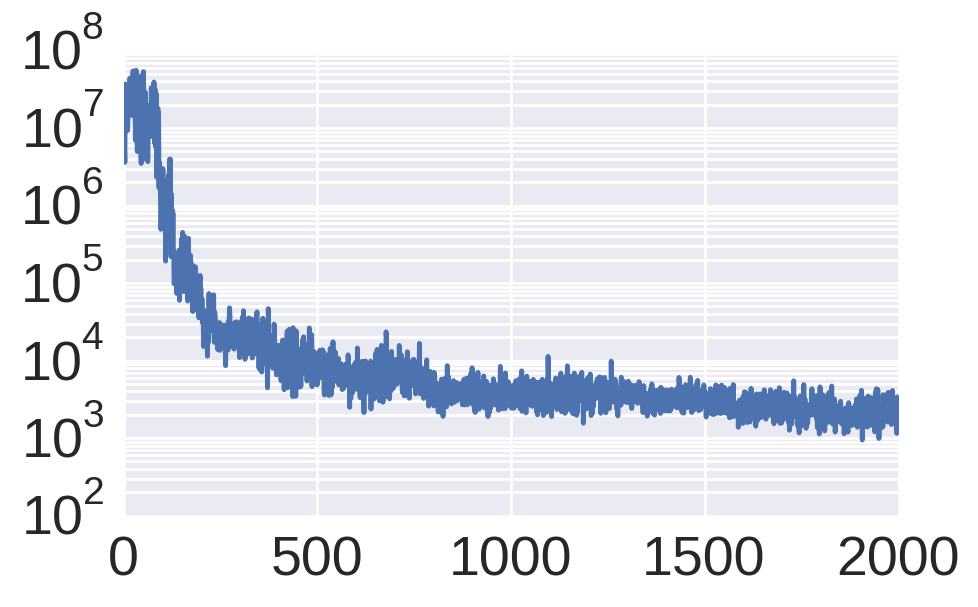
\includegraphics[height=4.5cm]{figs/structureAirline_res_c.png}
                \caption{Residuals}
                \label{fig:res}
        \end{subfigure}%
        ~ %add desired spacing between images, e. g. ~, \quad, \qquad, \hfill etc.
          %(or a blank line to force the subfigure onto a new line)
        \begin{subfigure}[b]{0.5\textwidth} \centering
                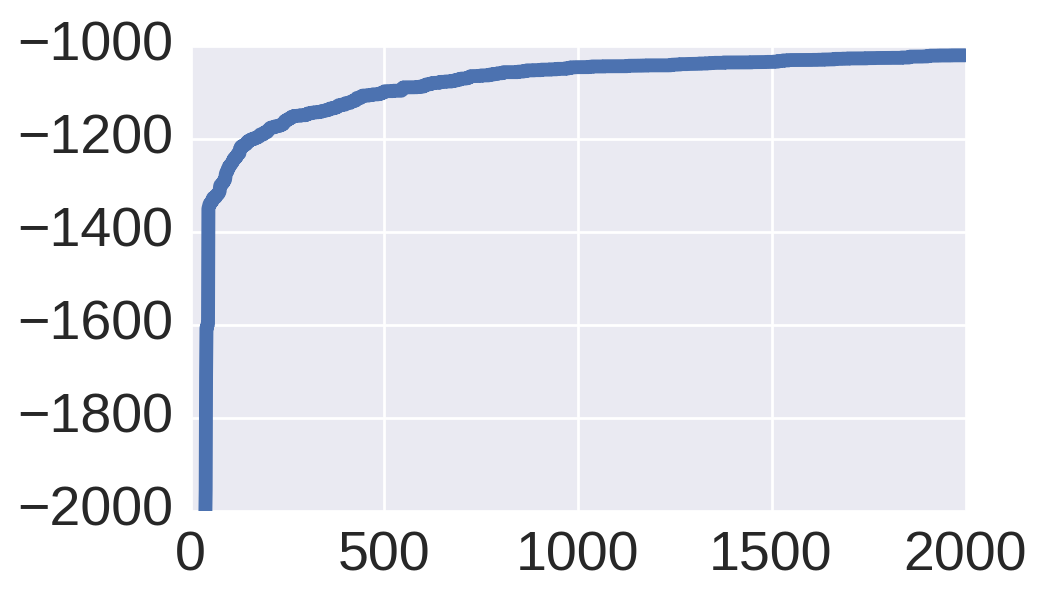
\includegraphics[height=4.5cm]{figs/structureAirline_log_c.png}
                \caption{Log Likelihood}
                \label{fig:log))}
        \end{subfigure}
        \caption{2000 steps along the Markov Chain.}\label{fig:reslog}
\end{figure}


Given two additive components $\mathbf{K} = \mathbf{K_a} + \mathbf{K_b}$, one can compute the margninal of a global component of a composite kernel structure~\citep{benavoli2015gaussian} with a gaussian posterior $\mathcal{N}(f_a \mid \hat{\mu}_a,\hat{\mathbf{K}}_a)$  where:

\begin{equation}
\label{eq:marginalComponentMean}
\hat{\bm\mu}_a   = \mathbf{K_a}(\xbf,\xbf^*)\, \mathbf{K}(\xbf^*,\xbf^*)^{-1}\, \ybf
\end{equation}
and covariance matrix
\begin{equation}
\label{eq:marginalComponentCovariance}
\hat{\mathbf{K}}_a =   \mathbf{K_a}(\xbf,\xbf) -  \mathbf{K_a}(\xbf,\xbf^*)\mathbf{K}(\xbf^*,\xbf^*)^{-1} \mathbf{K_a}(\xbf^*,\xbf).
\end{equation}
\end{comment}